\documentclass[9pt, aspectratio=169]{beamer}
%\documentclass[9pt, handout, aspectratio=169]{beamer} % makes just 1 slide for each frame (handout)

% language support
\usepackage[english]{babel}

% packages for figures
\usepackage{graphicx}
\usepackage{subcaption}

% math and physics packages
\usepackage{amssymb}
\usepackage{amsmath}
\usepackage{physics}
\usepackage{bm}
%\usepackage[compat=1.1.0]{tikz-feynman} % to create feynman diagrams

% other packages
\usepackage{multicol}
\usepackage{verbatim} % for the \begin{comment} command


% settings for theme/font
%%%%%%%%%%%%%%%%%%%%%%%%%
\usepackage{appendixnumberbeamer} % no page number in appendix
\usetheme[progressbar=frametitle]{metropolis}
\setbeamercolor{background canvas}{bg=white}
\usefonttheme[onlymath]{serif} % use "standard" font for math symbols
\setbeamertemplate{frametitle continuation}[from second][] % prevents numbering of content frame if it contains a frame break

\addtobeamertemplate{footline}{% add navigation bar and frame number at bottom
    \leavevmode
    \hbox{
    \begin{beamercolorbox}[wd=0.88\paperwidth,ht=2.75ex,dp=3.0ex,left,leftskip=1em]{}
        \usebeamercolor[fg]{navigation symbols}{\insertslidenavigationsymbol \insertframenavigationsymbol \insertsectionnavigationsymbol}
    \end{beamercolorbox}
    \begin{beamercolorbox}[wd=0.1\paperwidth,ht=2.5ex,dp=3.0ex,right,rightskip=1em]{footlinenum}
        \insertframenumber{} / \inserttotalframenumber
        \vskip 0.07pt
    \end{beamercolorbox}
    }
}{}


% Definitions of handy macros
%%%%%%%%%%%%%%%%%%%%%%%%%%%%%
\newcommand{\m}[1]{\mathrm{#1}}
\newcommand{\act}[1]{\action<+->{#1}}
\newcommand{\todo}[2][\huge]{\textcolor{red}{\fbox{#1#2}}} % to add red todo boxes
\newcommand<>{\uncoverubrace}[2]{% to cover/uncover underbraces
    \onslide#3 \underbrace{ \onslide<1->%
    #1%
    \onslide#3 }_{#2} \onslide<1->%
}

\let\phi\varphi
\let\epsilon\varepsilon

% to insert a tab
\newcommand{\tab}[0]{\phantom{1234}}




\title{Meron Cluster Algorithm for the 1+1 Dimensional $S=1/2$ Quantum Link Model}
%\subtitle{}
\author{Thea Budde}
\institute{ETH Zürich}
\date{20.3.23}




\begin{document}
\metroset{block=fill}

\begin{frame}
	\titlepage
\end{frame}

% frame with table of contents (which allows frame breaks)
\begin{frame}[allowframebreaks, t]
	\frametitle{Content}
	\setbeamertemplate{section in toc}[sections numbered]
    \tableofcontents
\end{frame}

\section{$S = 1/2$ Quantum Link Model}

\begin{frame}[t]{$S = 1/2$ Quantum Link Model}
    \begin{itemize}
        \item The $S = 1/2$ quantum link model is similar to the Schwinger Model, but with constrained field values
        \item A small derivation:
        \begin{itemize}
            \item Starting with the continuous Dirac Hamiltonian in 1+1 dimensions
            \begin{equation}
                H = \int d x \bar{\psi} (i \partial_\mu \gamma^\mu - m)\psi
            \end{equation}
            \item Discretize space and derivative to a finite volume $L = N a$
            \item Instead of placing a $2 \times 1$ spinor in each lattice site, a single fermion $c_n$ is inserted
            \item A spinor is then represented by two lattice sites
            \begin{equation}
                \psi_n = \frac{1}{\sqrt{a_{st}}} 
                \begin{pmatrix}
                    c_{2n} \\
                    c_{2n+1}
                \end{pmatrix}
            \end{equation}
            \item This is called staggered fermions and avoids the fermion doubling problem.
            \item The Hamiltonian becomes
            \begin{equation}
                H = \sum_{l=0}^{N-1} \left( - \frac{i}{2a} c_l^{\dagger}c_{l+1} + h.c. + m (-1)^l c_l^{\dagger} c_l \right).
            \end{equation}
        \end{itemize}
    \end{itemize}
\end{frame}

\begin{frame}[t]{$S = 1/2$ Quantum Link Model}
    \begin{itemize}
        \item Now introduce gauge field
        \item Want symmetry under $U(1)$ transformation $c_n \to e^{i\alpha_n} c_n$
        \item Introduce link variables such that $c_n^\dagger  U_{n,n+1} c_{n+1}$ is invariant
        \begin{align}\label{eq:transformation_properties}
            U_{n,n+1} \to e^{i\alpha_n}  U_{n,n+1} e^{-i\alpha_{n+1}}
        \end{align}
        \item Gauge field $L_n$ and $U_n$ are related through ? (not canonical conjugates themselves...)
        \item A gauge invariant Hamiltonian is given by
        \begin{equation}
            H = \frac{i}{2a} \sum_n (c_n^\dagger U_n c_{n+1}  - c_{n+1}^\dagger U_n^\dagger c_n ) + m \sum_n (-1)^n c_n^\dagger c_n + \frac{a e^2}{2} \sum_n L_n^2
        \end{equation}
    \end{itemize}
\end{frame}

\begin{frame}[t]{$S = 1/2$ Quantum Link Model}
    \begin{itemize}
        \item A gauge invariant Hamiltonian is given by
        \begin{equation}
            H = \frac{i}{2a} \sum_n (c_n^\dagger U_n c_{n+1}  - c_{n+1}^\dagger U_n^\dagger c_n ) + m \sum_n (-1)^n c_n^\dagger c_n + \frac{a e^2}{2} \sum_n L_n^2
        \end{equation}
        \item Gauge symmetry manifests in Generators $G_n$ that commute with the Hamiltonian
        \begin{equation}\label{eq:gauss_law}
            G_n = L_{n} - L_{n-1} - c_n^\dagger c_n + \frac{1 - (-1)^n}{2}.
        \end{equation}
        \item This is called Gauss's law and restricts physical configurations $G_n \ket{\psi} = 0$
        \item Gauss's law ensures that the difference between the left and right link of an
        \begin{itemize}
            \item even empty site is 1
            \item odd occupied site is -1
            \item even occupied and odd empty site is 0
        \end{itemize}
        \item The vacuum with a constant electric field is the configuration where all even sites are occupied and all odd sites are empty.
    \end{itemize}
\end{frame}

\section{Meron Cluster Algorithms}

\section{$S = 1/2$ Cluster Algorithm}

\section{Phase Transition}

\section{Outlook}



\section{Uncovering elements of a slide}


\begin{frame}[t]{"pause" command}
    Here I use the "$\backslash$pause" command
    \pause

    Next text
    \pause

    An equation
    \begin{equation*}
        E = mc^2
    \end{equation*}
    \pause
    Last text
\end{frame}



\begin{frame}[t]{Overlay specifications}
    \act{Here I use the "$\backslash$action" command or my macro $\backslash$act}

    \act{This is on the next slide}

    \action<3->{An equation} % Here I use action<3-> s.t. this text appears from the 3rd slide on together with the equation
    \begin{equation*}
        \act{1 = \frac{c^2}{c^2} = \frac{a^2 + b^2}{c^2}}
    \end{equation*}
    \action<4->{A multiline equation using the physics package}
    \begin{align*}
        \act{I &= \int_a^b x \dd{x}}
        \act{= \left[\frac{1}{2}x^2\right]_a^b}
        \act{= \frac{1}{2}\left(b^2 - a^2\right) \\}
        \act{&= \frac{1}{2}c^2 - a^2}
    \end{align*}
    \action<3, 7>{Because (This only appears on slide 3 and 7)
    \begin{equation*}
        a^2 + b^2 = c^2
    \end{equation*}}
\end{frame}

\begin{frame}[t]{Using underbraces}
    \action<1->{The underbraces only appear later}
    \begin{equation*}
        \act{E = \uncoverubrace<2->{\sqrt{p^2c^2 + m^2c^4}}{\text{Full expression}}}
    \end{equation*}
\end{frame}


\begin{frame}[t]{Figures and text}
    \begin{columns}
        \column{0.35\textwidth}
        \act{Column one with some text}
        \begin{itemize}[<+->]
            \item Item 1
            \item Item 2
        \end{itemize}

        \act{Some more text.}

        \act{Now one figure vanishes}

        \column{0.65\textwidth}
        \action<1->{% makes figures appear from 1st slide on
        \begin{figure}
            \centering
            \begin{subfigure}{0.49\textwidth}
            \centering
            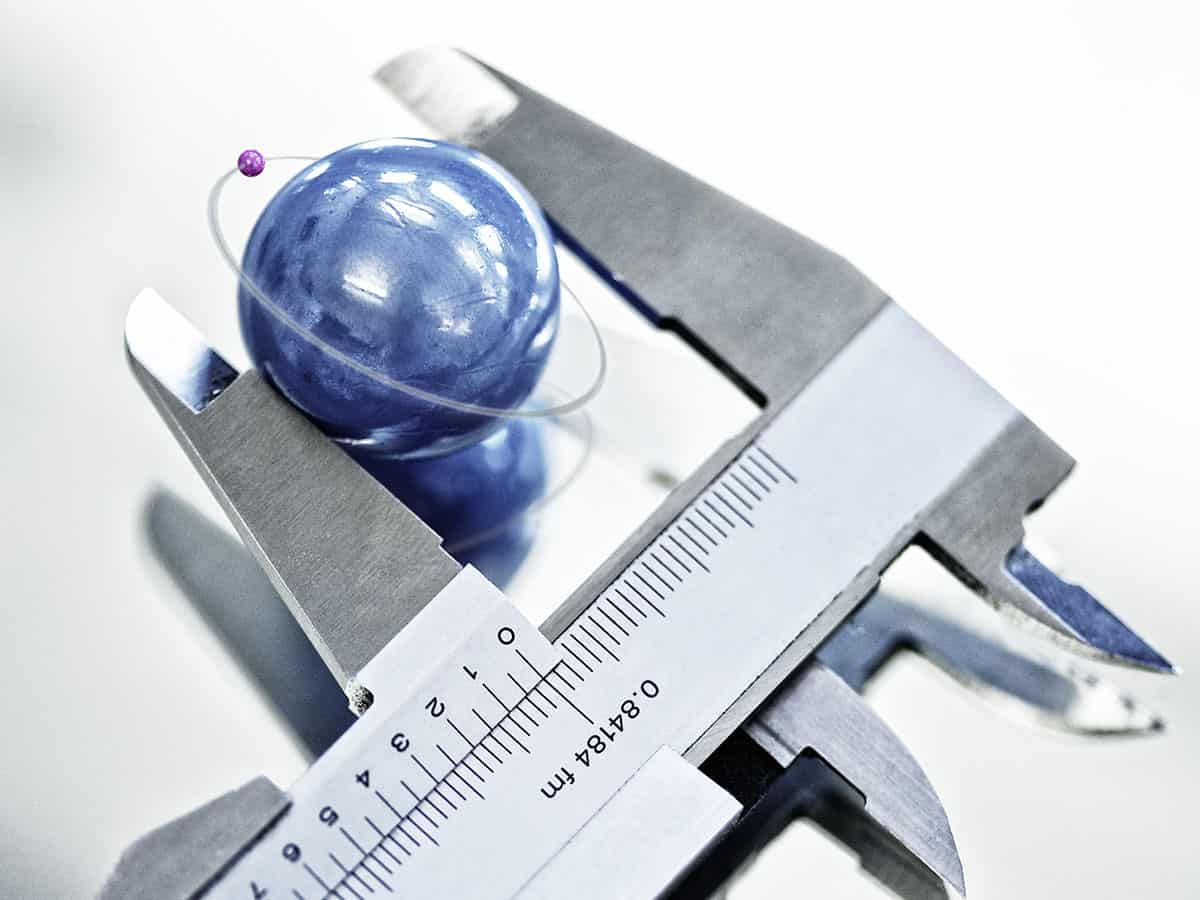
\includegraphics[width=0.87\textwidth]{Figures/proton_radius.jpg}
            \end{subfigure}
            \hfill
            \begin{subfigure}{0.49\textwidth}
            \centering
            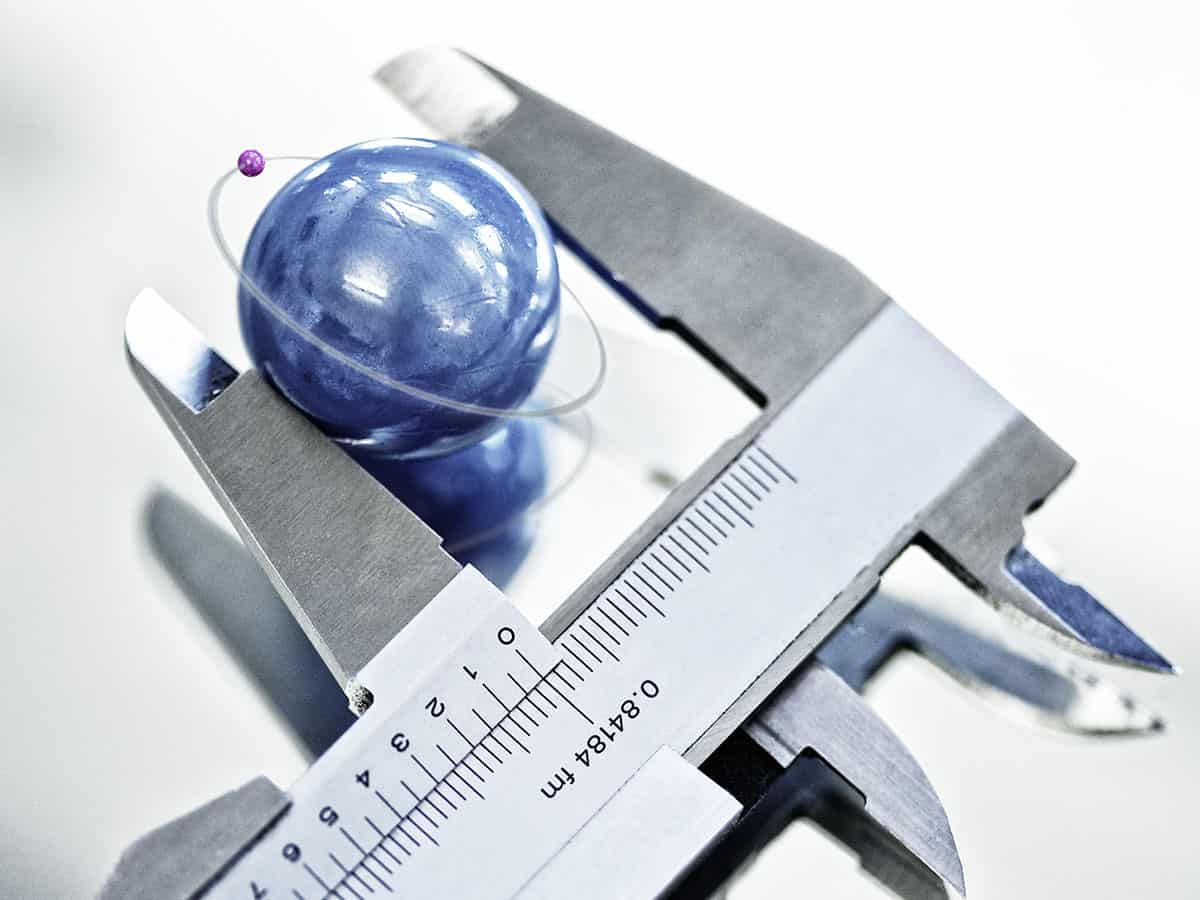
\includegraphics[width=0.87\textwidth]{Figures/proton_radius.jpg}
            \end{subfigure}
            \begin{subfigure}{0.49\textwidth}
            \centering
            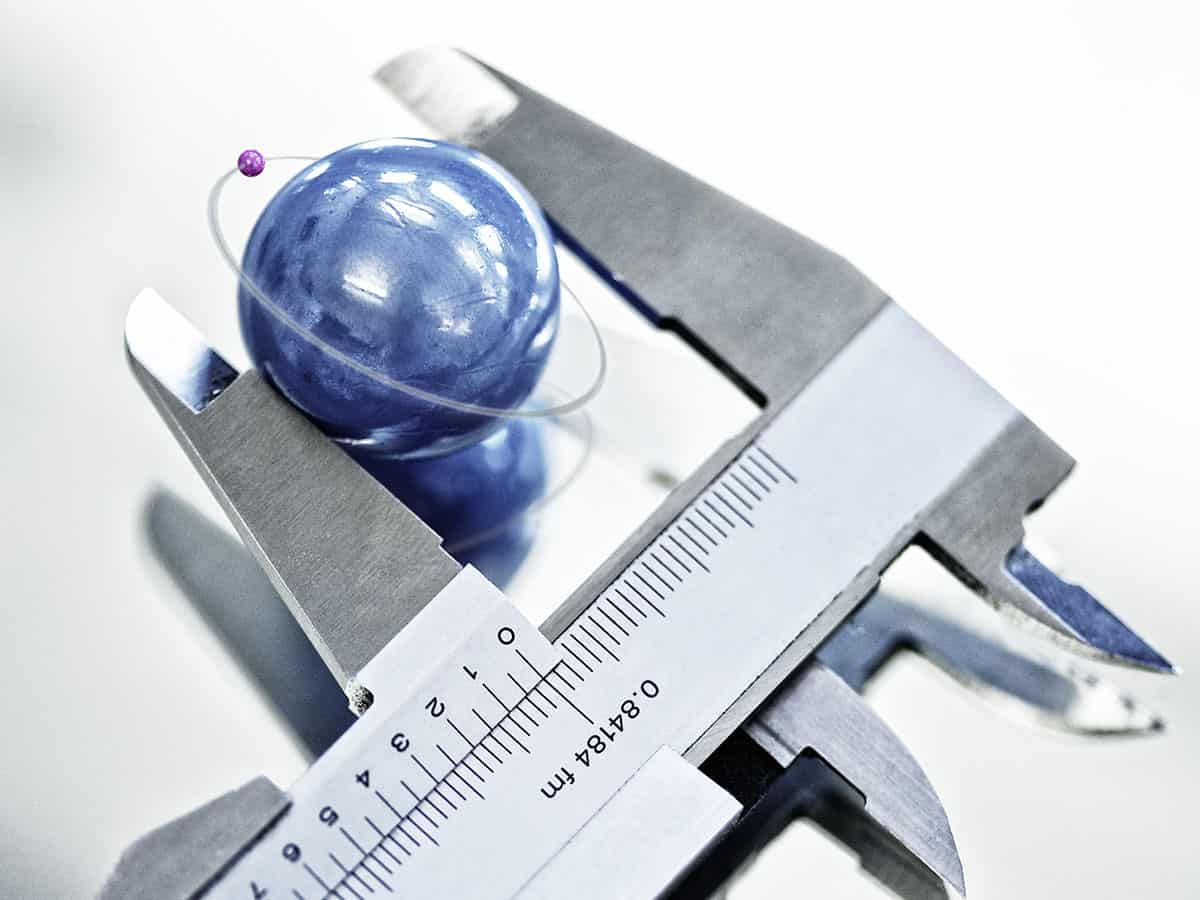
\includegraphics[width=0.87\textwidth]{Figures/proton_radius.jpg}
            \end{subfigure}
            \hfill
            \action<-4>{\begin{subfigure}{0.49\textwidth}
            \centering
            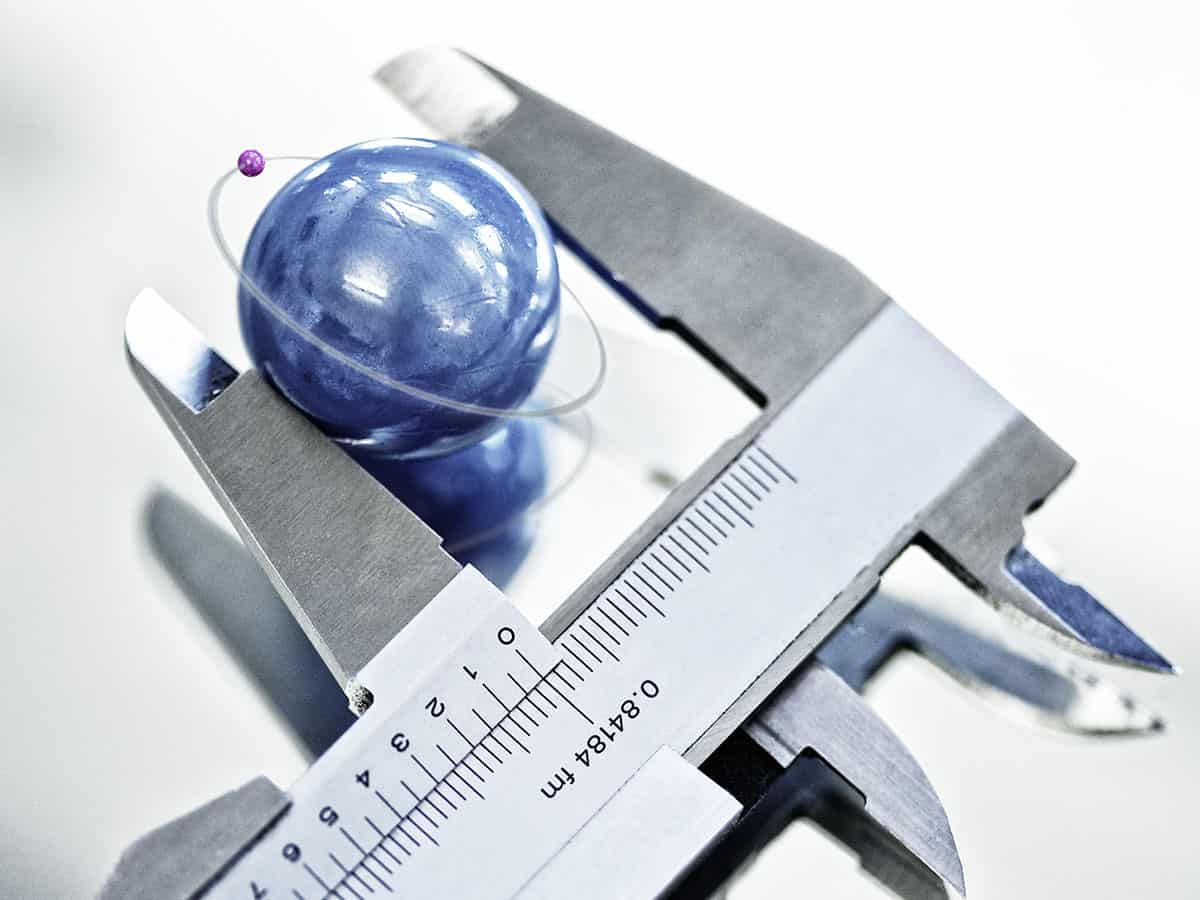
\includegraphics[width=0.87\textwidth]{Figures/proton_radius.jpg}
            \end{subfigure}}
        \end{figure}
        }
    \end{columns}
\end{frame}


\appendix

\section{Backup slides}

\begin{frame}[t]{Backup slide 1}
    This is a backup slide
\end{frame}

\begin{frame}[t]{Backup slide 2}
    This is the second backup slide
\end{frame}

\end{document}